\chaptertitle{2}{定投，做一个聪明的“懒人”}
\setcounter{figure}{0}\setcounter{table}{0}
其实定投这个概念我们并不陌生，很多人早就接触过了。比如，螺丝钉记得上小学的时候，就有银行员工到学校里宣传“教育储蓄”：给每个家长发传单，告诉家长们只要每隔一段时间存50元，将来孩子上高中大学的费用就攒出来了。

这种“零存整取”的思路就是定投的一种。

\subsection{什么是定投}
\subsubsection{五险一金，就是一种定投}

简单来说，定投就是“定期投入”的意思，把资金定期投入某个品种。

上班族，其实都在定投，比如平时缴纳的五险一金。

五险一金是养老保险、医疗保险、失业保险、工伤保险、生育保险和住房公积金的统称。

五险一金，也不全是上班族所负担的。实际上，每个月上班族需要自己缴纳的主要是养老保险、医疗保险、失业保险、住房公积金，并且其中很大比例是由单位负责缴纳。工伤保险和生育保险，则全部由单位缴纳。

一些单位为了节约成本，并没有帮助员工缴纳五险一金。这对员工来说是很大的损失，所以上班族要重视自己的五险一金。

五险一金所需的金额每个月自动从上班族的工资中扣除，所以每个月发到手的钱，其实已经扣掉了五险一金这部分金额。

每个月，工资发到手之后，我们看看工资条，里面有一部分就已经被自动拿出来投入了五险一金。这个过程会持续到我们退休。像我们投资的养老保险，国家就汇集成了养老基金来投资债券、股票。实际上大多数上班族都在用定投的方式每月来定投五险一金。

每个月在固定的时间拿一笔资金投入某个品种，这不就是一个定投的操作吗？

所以，我们大多数上班族，实际上都在坚持定投。

\subsubsection{定投，要投能带来现金流的资产}

定投的时候，我们要投资什么呢？

答案是可以产生现金流的资产。

什么是现金流呢？

螺丝钉给大家讲一个小故事，大家就明白了。

{\kaishu 从前有一个年轻的农夫，他每天的愿望就是从鹅笼里捡一个鹅蛋当早饭。结果有一天，他竟然在笼子里发现了一个金蛋。一开始，他不相信这是真的，他把这个金蛋拿给金匠看，金匠跟他说，这个蛋是由纯金铸成的。于是，农夫卖了这个金蛋，然后举行了一场盛大的庆祝会。}

{\kaishu 第二天，农夫一大早赶到鹅笼看，结果又发现一个金蛋躺在那里，这样的情况持续了好几天。}

{\kaishu 本来农夫可以靠着这只鹅从此过上好日子，可是这个农夫是一个贪婪的人，他对自己的鹅非常不满意，因为这只鹅没法向他解释是怎么下出金蛋的，否则他就可以自己制造金蛋了。农夫还气呼呼地想，这只懒惰的鹅每天至少应该下两个金蛋，现在这样的速度太慢了。}

{\kaishu 他的怒火越来越大，最后愤怒的农夫把鹅劈成了两半。从那以后，农夫再也得不到金蛋了。}

金蛋，就是我们手里的现金；而会下金蛋的鹅，则是我们的资产。

我们投资就是这样：能够产生现金流的才是资产，它就是我们的“鹅”，可以源源不断地给我们产生现金流。在日常生活中能产生现金流的资产有很多，像股票、债券、基金、房地产、自己的公司等，这些都是“鹅”。只要这只“鹅”可以产生不错的现金流，它就是在下“金蛋”。

\begin{itemize}
\item 债券，每年可以产生利息，利息是现金流。
\item 上市公司，每年可以产生盈利，盈利也是现金流。
\item 房地产，每年出租可以产生租金，租金也是现金流。
\item 我们自己上班工作，每个月可以领取工资，我们自己这个人力资产也可以产生现金流。
\item 我们自己经营了一家公司，这家公司正常运转，是赢利的，也可以给我们带来现金流。
\end{itemize}

只要拥有了足够多的“鹅”，即使我们不再工作，也可以源源不断地获取现金流，这是实现财务自由的很好方式。

说起来我们比这个故事里的农夫幸福很多，因为他只有一只下金蛋的鹅，而我们周围有许多可以下金蛋的“鹅”。我们可以努力工作，用工作所得来买“鹅”。在没有“鹅”的时候，这是一个很好的开始。

“千里之行，始于足下。”要积累大量的资产，有一个非常重要的前提，就是我们要有本金，有了本金我们才可以去买资产。所以获得第一桶金，是我们首先要做的。

越早开始积累资金用于投资，我们可以越早积累下资产。让资产为我们打工，不断地“钱生钱”，我们就可以更早地实现财务自由的目标。

日常生活中还有一些无法产生现金流的资产，比如黄金、古董、艺术品等。100年前囤下1公斤黄金，妥善保存到今天，仍然是1公斤黄金，不会有什么变化，黄金不会多出来。

不能产生现金流的资产，它的价格主要取决于供求关系。比如说在战乱年代，黄金通常会供不应求，价格上涨，所以才有“盛世珠宝，乱世黄金”的说法，所以有种说法是“黄金是避险资产”。但是在经济稳定发展的年代，黄金的投资价值并不高。图 \ref{fig:2-1} 为从1802年到2002年这200年，1美元投资于各类资产的变化。

\begin{figure}[htbp]
\centering
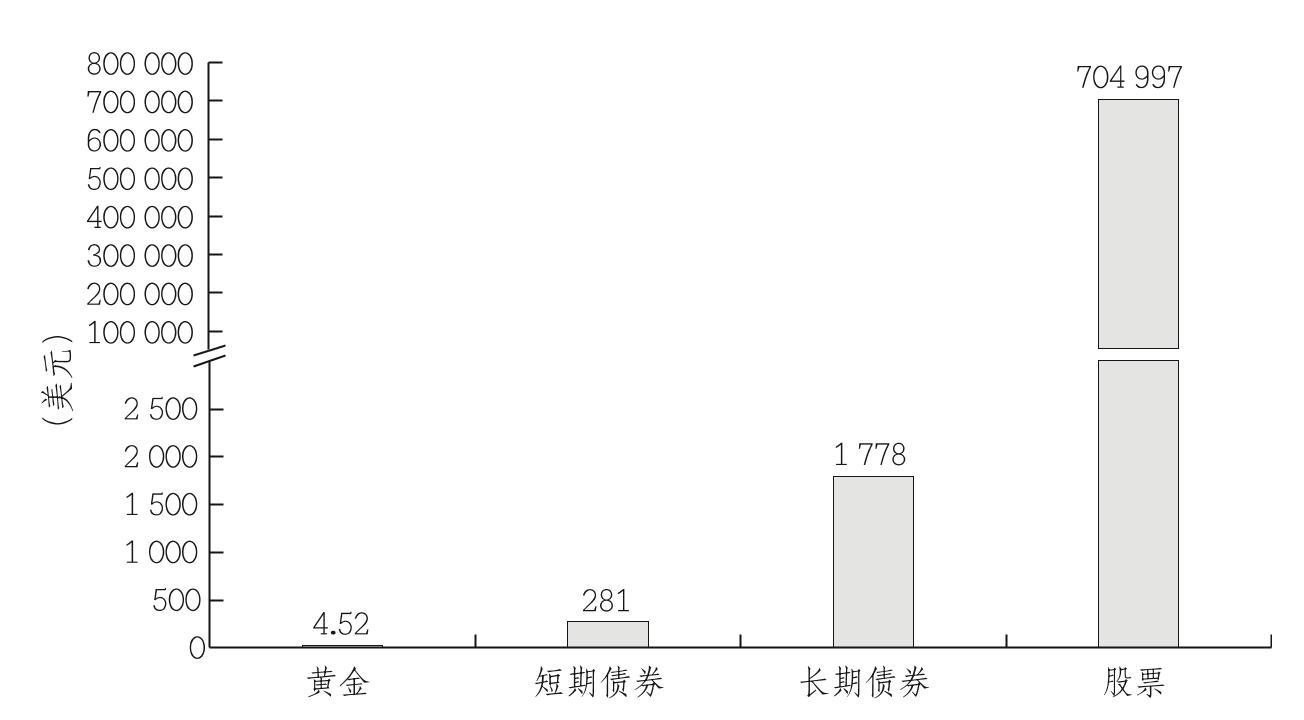
\includegraphics[width=\textwidth,height=0.82\textheight,keepaspectratio]{figure/图2.1.png}
\caption{1802—2002年，1美元投资于各类资产的变化}\label{fig:2-1}
\par\smallskip\noindent{\footnotesize 资料来源：杰里米·西格尔。《股市长线法宝》，马海涌等译，北京：机械工业出版社，2015。}
\end{figure}



我们可以看出，黄金的投资价值并不高，远远不如股票和债券。

这里有一个比较通用的概念：能产生现金流的资产通常比不能产生现金流的资产长期收益高；能产生现金流的资产中，现金流越高，长期收益越高。

所以，我们定投的时候，最好选择那些可以产生现金流的资产，这样长期收益才更高。

\subsection{定投的好处}
\subsubsection{定投的两个作用}

定投其实有两个非常重要的作用。

第一个作用，是强制储蓄，克服穷人思维。

大部分人无法区分消费和投资，因此需要有一个定期投入的操作，帮助他们积累资产。比如说单位发了1000元奖金，拿1000元买烟，这就是消费；但是如果用这1000元买基金，就是买了资产，进行投资。

表面上看起来，这两种都是花了1000元。但实际上抽烟完了就什么都不剩了；但是基金投资做好了，过段时间，投入的1000元就会增值，带来1000元之外的回报。

当然，投资的目的还是获得更多的财富，改善家庭的生活质量。

所以某种意义上，消费是把钱在当下就花掉；而投资是把钱投到某个品种上，期待未来获得更多的钱，然后在未来花掉。这就是消费和投资的区别。

成为富人的第一步，就是要明白消费和投资的区别。绝大多数人都是卡在了这一步。很多人区分不了消费和投资，或者无法忍耐长时间等待投资收益。

我们身边都有这样的“月光族”。他们没有自己的规划，到手的钱基本都会花掉，甚至还会借钱消费，部分人还可能欠下巨债。如果社会上人人都如此，肯定不利于社会的安定，所以国家强制让大家做五险一金的定投。

同样地，我们也可以用类似的方式制订一个定投计划，帮助自己强制储蓄。如果觉得自己积累不下财富，那就来定投吧。

第二个作用，是保值增值，化解人力资产的风险。

我们年轻的时候可能都需要依靠自己的体力或者努力工作来赚取工资收入。这其实是把自己这个人力资产运作起来产生现金流。

如果每个月我们把一部分现金流转换成其他资产，持续几十年的时间。等到积累的资产足够多，这些资产产生的现金流可以覆盖我们家庭日常生活的开销，也就实现财务自由了。

这就是用定投来化解人力资产的时间风险。

\subsubsection{定投最适合的四类人群}

有四类人群，很适合用定投的方式来进行投资。分别是上班族、大忙人、低风险投资者和为未来规划者。

第一类，也是最典型的，就是上班族。定投，可以说是为上班族量身定做的。上班族每个月会获取一定的工资收入，这些收入的结余部分可以定期投入指数基金，获取更高的收益。国家让上班族用定投的方式缴纳社保和养老保险，就是因为这个方法特别适合上班族。

第二类，是大忙人。定投不需要盯盘，每个月只需要在固定的某一天，抽出几分钟判断一下所关注的指数基金是否值得投资即可。甚至可以设置自动定投，连理都不用理，隔一段时间查看一下收益即可。当然，配合本书介绍的定投策略，需要在每月定投的时候先判断当前情况下指数基金是否仍然值得继续投资，只有值得投资时，我们才继续定投，所以最好是手动操作。

第三类，是低风险投资者。股票基金波动性比较大，如果一次性买入，很可能遭遇大幅暴跌。但是定投，通过分批买入的方式可以降低风险，如果买在相对高点，之后的定投会把我们的买入成本降下来。因此，定投非常适合追求稳健的低风险投资者。

第四类，是为未来规划者。定投类似于零存整取，适合为未来特定的目的做规划。同时，定投又优于零存整取，我们可以将平时不用的闲钱整合起来，持续获取高收益。例如，作为未来买房的首付款、将来孩子上学的教育款，或是退休之后的养老费用等。

\subsubsection{定投的收益}

最倒霉的定投者，这是杰里米·西格尔（Jeremy Siegel）教授在他的著作《股市长线法宝》中讲过的一个人物。

{\kaishu 1929年6月，一个新闻记者采访了当时通用汽车公司（General Motors）的高级财务总监拉斯科布。拉斯科布讲了一个比较大胆的观点：人人都能发财。}

{\kaishu 在访谈里，拉斯科布说，投资者只需要每个月定投15美元，投入美国股市，在未来的20年里，投资者的财富有望稳步增长至8万美元。}

{\kaishu 当时正好是美国股市的牛市，在20世纪20年代的牛市狂热氛围中，几乎没有人怀疑这个言论。}

{\kaishu 但是在拉斯科布发表观点7周之后，美股股市崩盘，34个月之后，道琼斯指数（Dow Jones Industrial Average，简称DJIA）只剩下41点。}

{\kaishu 大盘股的市值蒸发了89\%，数百万投资者的毕生积蓄化为乌有，美国经济进入历史上最严重的萧条期。}

{\kaishu 毫无疑问，拉斯科布的言论遭到了无情嘲讽和抨击，甚至有议员说拉斯科布让普通民众在市场顶部买入股票，应该为股市崩盘承担责任。《福布斯》（Forbes）专门撰文指责嘲讽拉斯科布。}

{\kaishu 拉斯科布错了吗？}

{\kaishu 事实上，如果一个投资者在1929年按照拉斯科布的建议构建长期定投组合，每个月坚持定投15美元到美国股市，我们可以计算一下该组合的收益。}

\begin{itemize}
\item {\kaishu 到1949年，累计资金将达到9000美元，年化收益率为7.86\%，高出当时债券收益率两倍以上。}
\item {\kaishu 30年后，累计资金将增加至6万美元以上，年化收益率也上涨到12.72\%。}
\end{itemize}

{\kaishu 尽管没有拉斯科布预测的那么高，但也是同期债券年化收益率的8倍以上了。}

{\kaishu 为什么会这样呢？因为下跌之后，美国股市从股灾后又涨了回来，而且涨得更高。}

拉斯科布可谓是最倒霉的定投者了。但即使像拉斯科布这样倒霉，在牛市的最高点开始，经历了有史以来最严重的股市崩盘，定投也可以帮助他取得不错的收益。

假如他能在定投的时候看一下股市的估值，在股市低估的时候才开始定投，长期来看会有一个更加惊人的投资业绩。而这种方法，正是本书后面将要介绍给大家的投资方法。

再比如我们制订了以下简单的定投计划。

{\kaishu 例如我们在某场外基金交易平台，每个月的第一天，定投1000元到沪深300指数基金。}

这样一个定投方案的效果如何呢？

我们借用定投计算器来回测一下。

时间最久的一只沪深300指数基金，成立于2003年8月。我们以这只沪深300指数基金为例。

{\kaishu 从2003年9月1日开始，每月1日，定投1000元至沪深300指数基金。截至2019年4月19日，一共执行188期定投，投入188000元。累计持有的基金总市值是448919元，约45万元，累计收益率138.79\%。}

这个收益意味着什么呢？

如果我们同期定投的是一只年化收益率为3\%的货币基金，那么定投188期下来，累计持有资产大约23万元。

如果同期定投的是一款年化收益率为5\%的银行理财产品，那么定投188期下来，累计持有资产大约28万元。

如果同期定投的是一款年化收益率为10\%的高收益产品，那么定投188期下来，累计持有资产大约43万元，略低于定投沪深300指数基金。

所以，仅仅是简单定投沪深300指数基金，不添加任何策略，效果比定投一款年化收益率为10\%的理财产品还要好，积累家庭财富的速度也更快。

这就是定投指数基金的好处。我们只需每个月拿出一点点时间，进行指数基金的定投，就可以获得这样的好收益。

再分享一个中国香港居民定投指数基金的案例。

{\kaishu 一个普通的香港打工仔，他一辈子的收入都是普普通通的中位数。}

{\kaishu 假如他从1964年18岁开始工作，每年拿出收入的20\%投资恒生指数基金，那他每年的投入，会从500多元慢慢增长到2万多万。到他58岁退休时（2004年），他将拥有660万元的资产。}

{\kaishu 如果他到2014年也就是68岁才退休，他就可以拥有1576万元的资产。而要完成这一切，他定投的本金总共只需65万元而已！}

{\kaishu 仅仅是年复一年的定投，累积定投65万元，退休的时候就会有1500多万元的资产。这还只是一个人，如果是双职工家庭，退休时很轻松可以存下3100万元的资产。}

{\kaishu 这就是定投指数基金的威力。而掌握这些不需要有多么高深的投资技巧，只需要年复一年地从收入中拿出一部分用来定投就可以。}

不过，相信大家还是有一些疑惑。

（1）定投具体的操作步骤是什么？

（2）指数基金品种那么多，该选择哪只指数基金来投资呢？

（3）定投指数基金长期下来收益不错，为何我身边还是有很多朋友投资指数基金是亏损的呢？

（4）这个定投方法这么简单有效，那还有没有更优化、让我们获得更好收益的方法呢？

在接下来的章节，螺丝钉将会给大家介绍投资指数基金的具体操作步骤，以及螺丝钉自己精心总结的提高定投收益的非常有用的技巧。这些技巧都是经过多年实践经验和几十万投资者的验证得的，可以很好地帮助我们提高定投指数基金的收益。

\subsection{定投的心态，就像还房贷}
\subsubsection{定投是一种被动投资理念：不要去预测市场}

经常有朋友问螺丝钉以下问题。

{\kaishu 看到股市下跌很兴奋，但还没有到我定投的日子，我怕到时候就涨上去了，所以可不可以先投一点呢？}

这样的想法，到底对不对呢？

其实，产生了这样的想法，就说明投资者心里是如下这样认定的。

{\kaishu 当前时刻就是这个月最便宜的时候，后面的时间段里，不会再下跌，不会再出现更便宜的价格了。}

因为，如果认为后面还会下跌，是不会想着现在就投资的。这其实是一种依靠主观来判断短期涨跌的行为。

而一般情况下，都不建议大家凭主观去判断股市涨跌，因为很少有人能长期准确地判断出股市短期的涨跌，大多数人都不具备这样的能力。如果真有这样的人，肯定已经家喻户晓了。所以凭主观去判断要不要加仓，也许偶尔会成功几次，但长期的成功是无法保证的。

所以，我们才会采用“定投”这种投资方式，摒弃人的主观判断，承认自己“无法准确判断短期市场的涨跌”。选择这种定期投资的方式，是更加稳妥的。

对大多数投资者来说，在一个固定的时间点进行投资，可以避免主观情绪的干扰，反而效果更好。

\subsubsection{定投就像还房贷}

其实仔细想一想，我们定投跟还房贷挺像的。还房贷是一件挺有意思的事情。

\subsubsection{还房贷的那些事儿}

首先，我们每个月到了约定的时间点，就要把钱准备好，用来还款。

其次，虽然房价有涨有跌，但我们不敢推迟还货款，因为一旦逾期被计入征信系统，后面办理很多事情时都会有麻烦。

但通常来说，我们也不想每个月提前还贷款，因为钱放在自己手上至少还可能有一点儿利息。所以，最好的策略就是每个月在还款日之前，找一个临近的固定时间点来还。

最后，当我们还完贷款之后，手里就拥有一套房子这样的资产了。

可以看出，还房贷其实是一次纪律性很完美的定投。在每个月固定的时间点还贷款，不会滞后，也不会提前。每个月还多少钱也会精心设计好。长期坚持下来，手里就有了一套房子。

\subsubsection{定投的那些事儿}

再来看看我们定投的情况。

首先，每个月到了时间点就进行定投。

其次，我们无法判断股市短期的涨跌，提前定投或者推迟定投都不能保证效果就比到了定投日进行定投更好。所以，最好的策略就是每个月到了自己计划好的定投日，进行定投。

这样长期坚持下来，我们手里就会积累大量的“钱生钱”资产。

\subsubsection{定投与还房贷的区别}

定投和还房贷的模型差不多，都是“聚沙成塔”。但是区别在于：房子这种资产具有使用价值，先把资产给我们使用，后面再慢慢还款。定投则是慢慢投资，逐渐积累起资产。

那么我们需要攒下多少资产，才能实现财务自由呢？

我们下一章再讲。

\subsubsection{投资者笔记}

\begin{itemize}
\item {\kaishu 定投就是“定期投入”的意思，把资金定期投入某个品种。}
\item {\kaishu 能够产生现金流的才是资产，它就是我们的“鹅”，可以源源不断地给我们产生现金流。只要拥有足够多的“鹅”，即使不再工作，我们也可以源源不断地获取现金流，这就是实现财务自由的很好方式。}
\item {\kaishu 定投，最适合这四类人群：上班族、大忙人、低风险投资者和为未来规划者。}
\item {\kaishu 对大多数投资者来说，在一个固定的时间点进行投资，这样可以避免主观情绪的干扰，效果更好。}
\end{itemize}
